\subsubsection{Interfaz Humano - Máquina}

Para la interfaz humano - máquina, es necesario utilizar algún tipo de pantalla que permita mandar información sobre el proceso de compostaje al usuario. Con este antecedente, se buscó alguna pantalla donde se puedan mostrar los mensajes de l forma mas eficiente posible.

\begin{table}[h!]
    \centering
    \caption{Características de la Pantalla LCD 20X4}
        \begin{tabular}{ |c|c|c|c| } 
            \hline
            \multirow{5}{8em}{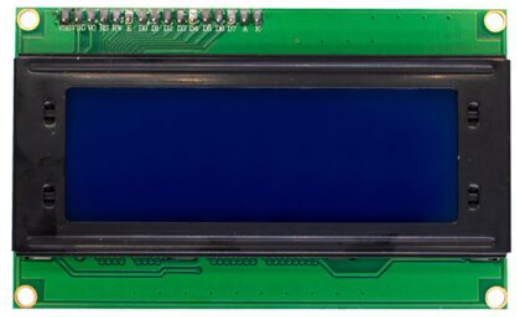
\includegraphics[scale=0.17]{images/Capitulo 4/3.1.1/S1/lcd2x4.png}} & \cellcolor[rgb]{ .851,  .851,  .851}Alimentación & \cellcolor[rgb]{ .851,  .851,  .851} 5 V \\ 
            & Tecnología & LCD \\ 
            & \cellcolor[rgb]{ .851,  .851,  .851}Corriente de operación & \cellcolor[rgb]{ .851,  .851,  .851} 125 mA \\ 
            & Puerto de comunicación & I2C \\
            & \cellcolor[rgb]{ .851,  .851,  .851}Dimensiones & \cellcolor[rgb]{ .851,  .851,  .851} 98 x 60  mm \\
             \hline
        \end{tabular}
    \label{tab:LCD CAR}%
\end{table}

A partir de esta comparación, se ha seleccionado la Pantalla LCD 20 X4 (tabla \ref{tab:LCD CAR}), esta pantalla es de un tamaño considerable por lo que se puede desplegar mas información al mismo tiempo. Esta pantalla incluye un módulo I2C, el cual disminuye el número de pines que se conectan entre la tarjeta de desarrollo y la pantalla, pasando de 8 pines a solamente 2.

Esta pantalla tiene el mismo principio de funcionamiento que su equivalente 16x2, por lo que es muy fácil integrarla a la programación principal. 

Otro aspecto que se consideró para la interfaz, es un juego de botones, que serán los encargados de recibir las indicaciones del usuario. Para efectos prácticos, se tiene planeado que cada uno de los botones cumpla con una función en específico de la siguiente manera:

\begin{enumerate}
    \item Botón 1: Arranque del sistema de compostaje
    \item Botón 2: Mostrar el valor de cada variable del ambiente físico del sistema.
    \item Botón 3: Mostrar información de la etapa de compostaje
    \item Botón 4: Tiempo de proceso de compostaje
\end{enumerate}

Aquí se hizo una revisión de los diferentes tipos de botones que existen en el mercado y se ha seleccionado uno, por criterios de accesibilidad, costo e integración con el chasis de la interfaz. La opción que se selecciono es el botón con membrana  incluida cuyas características se muestran en la tabla \ref{tab:Boton CAR}.

\begin{table}[h!]
    \centering
    \caption{Características de los botones de la interfaz}
        \begin{tabular}{ |c|c|c|c| } 
            \hline
            \multirow{5}{8em}{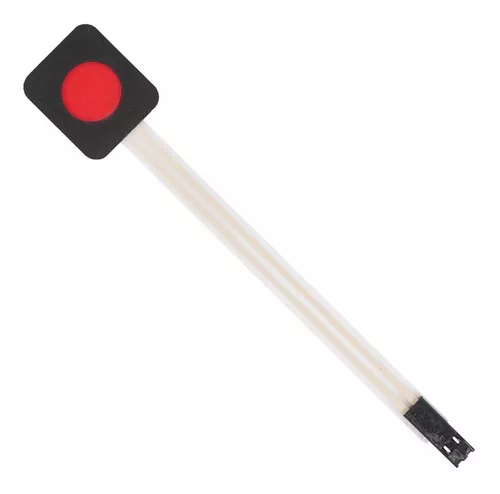
\includegraphics[scale=0.15]{images/Capitulo 4/3.1.1/S1/membrana.png}} & \cellcolor[rgb]{ .851,  .851,  .851} Tipo de contacto & \cellcolor[rgb]{ .851,  .851,  .851} Normalmente abierto \\ 
            & Colores & Verde, rojo y amarillo \\ 
            & \cellcolor[rgb]{ .851,  .851,  .851}Conexión & \cellcolor[rgb]{ .851,  .851,  .851} Cable dupont \\ 
            & Montaje en el chasis & Pegatina \\
            & \cellcolor[rgb]{ .851,  .851,  .851}Dimensiones & \cellcolor[rgb]{ .851,  .851,  .851} 23 x 20  mm \\
             \hline
        \end{tabular}
    \label{tab:Boton CAR}%
\end{table}

Debido a que el interruptor está normalmente abierto, se va a conectar en configuración de pull up (Figura \ref{fg:pullup}). Esta configuración es para mandar señales lógicas altas (1 lógico), de esta forma, activar la opción seleccionada.

\begin{figure}[h!]
            \centering
            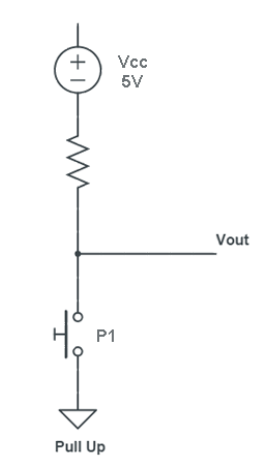
\includegraphics[scale=0.3]{images/Capitulo 4/3.1.1/S1/conexion.png}
            \caption{Configuración Pull Up}
            \label{fg:pullup}
        \end{figure}

De esta manera se trazo el circuito electrónico de la interfaz (Figura \ref{fg:SQ Interfaz}), en el cual se toman en cuenta la tarjeta ESP 32, el conector I2C de la pantalla LCD 20x4 y los 3 botones.

\begin{figure}[h!]
            \centering
            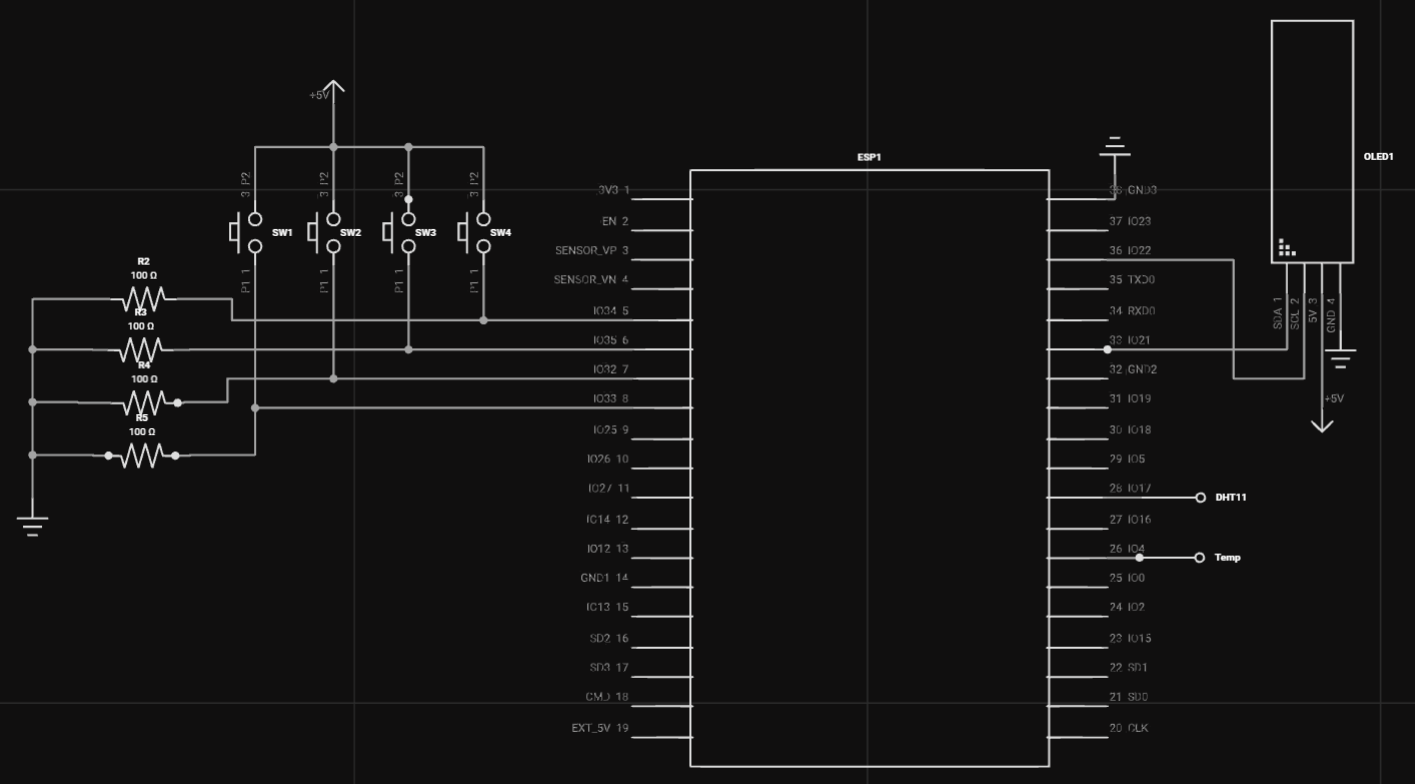
\includegraphics[scale=0.3]{images/Capitulo 4/3.1.1/S1/Interfaz cto.png}
            \caption{Circuito esquemático de la interfaz}
            \label{fg:SQ Interfaz}
        \end{figure}

        \newpage